% ------------------------------------------------------------------------------
% TYPO3 CMS 7.3 - What's New - Chapter "Backend User Interface" (English Version)
%
% @author	Michael Schams <schams.net>
% @license	Creative Commons BY-NC-SA 3.0
% @link		http://typo3.org/download/release-notes/whats-new/
% @language	English
% ------------------------------------------------------------------------------
% LTXE-CHAPTER-UID:		cc6b358d-f0ed36d3-f7a72fa2-af63ccfc
% LTXE-CHAPTER-NAME:	Backend User Interface
% ------------------------------------------------------------------------------
% LTXE-SLIDE-START
% LTXE-SLIDE-UID:		111332b8-ac46a07a-319ed582-f873bc02
% LTXE-SLIDE-ORIGIN:	b4dc1576-57b4854f-26a32d85-11f7c52b German
% LTXE-SLIDE-TITLE:		Feature #66173: Allow page title edit by doubleclick
% LTXE-SLIDE-REFERENCE:	Feature-66173-AllowPageTitleEditByDoubleclick.rst
% ------------------------------------------------------------------------------
\begin{frame}[fragile]
	\frametitle{Backend User Interface}
	\framesubtitle{Page Title in Page- and List-Module}

	Users can edit page titles in the "Page" and "List" module by double-clicking the page
	header or the edit icon.

	\begin{figure}
		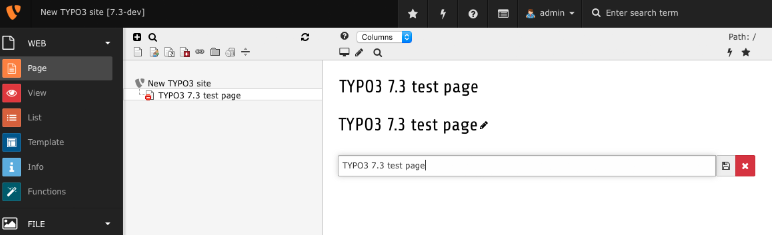
\includegraphics[width=0.9\linewidth]{BackendUserInterface/66173.png}
	\end{figure}

\end{frame}

% ------------------------------------------------------------------------------
% LTXE-SLIDE-START
% LTXE-SLIDE-UID:		c17b263e-12512d4b-13d5389f-df1ec14e
% LTXE-SLIDE-ORIGIN:	168b1424-1ebb2552-ed5bac3e-8a9ac737 German
% LTXE-SLIDE-TITLE:		Feature #67071: Processed files cleanup tool added in Install Tool
% LTXE-SLIDE-REFERENCE:	Feature-67071-ProcessedFilesCleanupToolAddedInInstallTool.rst
% ------------------------------------------------------------------------------
\begin{frame}[fragile]
	\frametitle{Backend User Interface}
	\framesubtitle{Install Tool: Delete Processed Files}

	In its "Clean up" section, the Install Tool provides a new function to remove
	processed files (e.g. image thumbnails) from FAL now.\newline
	This is useful if graphic-related settings have been changed or after an update of
	GraphicsMagick/ImageMagick to force all images to be regenerated.

	\begin{figure}
		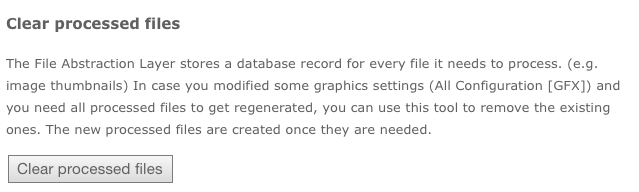
\includegraphics[width=0.6\linewidth]{BackendUserInterface/67071.png}
	\end{figure}

\end{frame}

% ------------------------------------------------------------------------------
% LTXE-SLIDE-START
% LTXE-SLIDE-UID:		4662a0fc-e8a91f22-2f75e0bc-800e9b63
% LTXE-SLIDE-ORIGIN:	daa83c1e-08d2716b-de74cbda-42361551 German
% LTXE-SLIDE-TITLE:		Feature #67319: Add field "copyright" to EXT:filemetadata
% LTXE-SLIDE-REFERENCE:	Feature-67319-AddFieldCopyrightToEXTfilemetadata.rst
% ------------------------------------------------------------------------------
\begin{frame}[fragile]
	\frametitle{Backend User Interface}
	\framesubtitle{New Field in FAL Meta Data}

	The field "\textbf{Copyright}" has been added to the meta data of a FAL record
	(system extension: \texttt{filemetadata}).

	\begin{figure}
		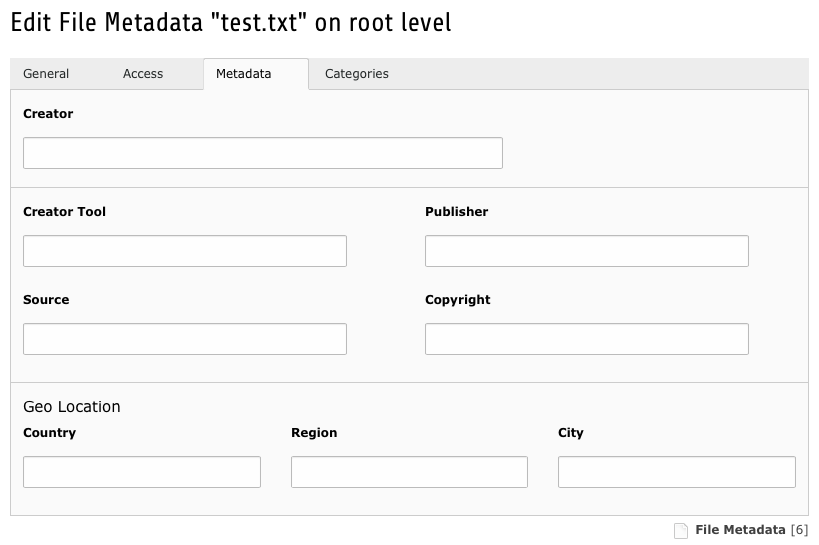
\includegraphics[width=0.6\linewidth]{BackendUserInterface/67319.png}
	\end{figure}

\end{frame}

% ------------------------------------------------------------------------------
